\chapter{Parte 1}
\label{cap:p1}

\section{Análise do problema}

Nesta 1ª parte do trabalho, pretende-se criar um modelo que permita descobrir
o caminho mais longo de um grafo orientado acíclico. Visto que neste grafo em
particular os nós correspondem a atividades e as arestas unidirecionais traduzem
as precedências entre as atividades, a rede pode ser entendida como um projeto,
cujas atividades devem ser realizadas obedecendo à ordem das suas precedências.
Neste contexto, encontrar o caminho mais longo significa por isso encontrar
a duração mínima do projeto.

\begin{figure}[<+htpb+>]
	\centering
	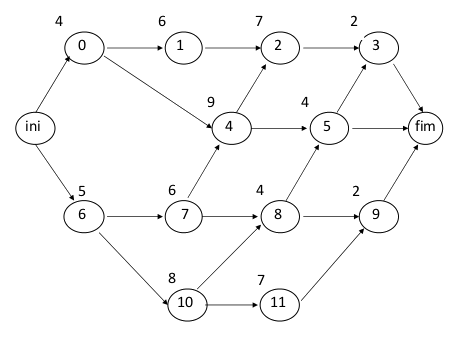
\includegraphics[scale=0.5]{./img/p1_rede_original}
	\caption{Grafo Inicial do enunciado}
	\label{p1:fig:rede_original}
\end{figure}

Antes de partir para a formulação do modelo, foi necessário saber qual a rede
a considerar. À rede fornecida no enunciado (figura \ref{p1:fig:rede_original}) foi necessário retirar dois nós, de
acordo com a metodologia apresentada na secção \textit{Determinação da Lista de
Atividades} presente no final do enunciado. Os números de aluno dos autores
deste relatório são 61778, 71164 e 72628. Como o número mais alto é 72628, então
D=2 e E=8, sendo por isso os nodos 2 e 8 a ser retirados da rede. A rede
resultante da remoção destes dois nós tem a representação gráfica mostrada na figura \ref{p1:fig:rede_com_duracoes}:

\begin{figure}[<+htpb+>]
	\centering
	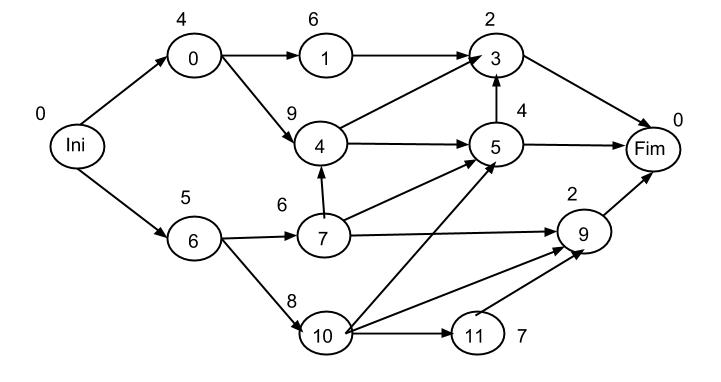
\includegraphics[scale=0.5]{./img/p1_rede_com_duracoes}
	\caption{Grafo resultante da remoção das atividades 2 e 8, com indicação da duração de cada atividade (em unidades de tempo arbitrárias)}
	\label{p1:fig:rede_com_duracoes}
\end{figure}

\newpage
\section{Modelo}

\subsection{Parâmetros}

Os parâmetros deste modelo são as precedências e as durações de cada atividade.

\subsection{Variáveis de decisão}
\label{p1:subsec:vardec}

O modelo desenvolvido nesta primeira parte tem como objetivo achar o caminho
mais longo da rede. Visto que se pretende achar um caminho, cada arco do grafo terá
associada uma variável de decisão, que tomará o valor de 1 ou 0, caso esse arco
faça ou não parte do caminho mais longo, respetivamente. As variáveis de
decisão serão por isso binárias. Embora a restrição relativamente ao fato das variáveis serem binárias não se encontrar explícita no modelo, ela é garantida por características específicas deste modelo que serão detalhadas na secção \ref{p1:sec:restricoes}.

Relativamente à nomenclatura das variáveis,
usou-se $X_{I\_J}$ para representar a aresta que vai da atividade I para
a atividade J. Assim, $X_{2\_4}$ representa a aresta que vai da atividade 2 para
a atividade 4.

\subsection{Função objetivo}

Como se pretende achar o caminho mais longo, a função objetivo terá que ser uma
expressão que indique a duração de um caminho, que queremos que tome o maior
valor possível. Trata-se por isso de um problema de maximização.

Visto que os valores das variáveis de decisão indicam os arcos que fazem ou não
parte de um caminho, para se construir a função objetivo com essas variáveis,
foi necessário associar um custo a cada um dos arcos. A decisão tomada foi a de
assumir que cada arco tem um custo correspondente à duração da atividade de onde
esse arco é originado. Por exemplo, o arco $X_{0\_1}$ tem origem na atividade
0 e destino na atividade 1, e terá um custo de 4, visto ser essa a duração da
atividade 0. O sentido em termos práticos de assumir que a duração não está na atividade mas sim nas arestas do grafo que dele saem  corresponde a dizer que a atividade em si não tem duração, o que tem duração é sim a passagem dessa atividade para uma outra. Embora isto possa ser pouco intuitivo em termos reais, esta consideração revela-se extremamente útil para a resolução do modelo como veremos de seguida.

Em qualquer solução admissível, o custo de um arco só deverá ter influencia no
valor da função objetivo se o arco fizer parte do caminho. Uma vez que as
variáveis de decisão traduzem com 1 ou 0 o facto de o arco fazer ou não parte do
caminho, então para saber o custo efetivo de um arco numa determinada solução,
basta multiplicar o seu custo pela variável de decisão associada. Designando por $C_{I}$ esse custo efetivo, temos a seguinte expressão:

\begin{displaymath}
C_{I} = C_{I\_J} \times X_{I\_J}
\end{displaymath}

Onde:
\begin{description}
	\item[$C_{I\_J}$] Custo associado ao arco que vai de I para J - parâmetro do problema
	\item[$X_{I\_J}$] Variável de decisão indicativa se o arco faz ou não parte do
	caminho, conforme detalhado na secção~\ref{p1:subsec:vardec}.
\end{description}

Esta multiplicação faz sentido, uma vez que tanto as variáveis de decisão como as durações das atividades estão associadas aos arcos. Tal mostra a utilidade em termos de resolução de modelo de anteriormente se ter associado a duração das atividades aos arcos.

A função objetivo será o somatório de todos esses custos. Em termos genéricos, pode ser
escrita como:

\begin{displaymath}
\max~z = \sum C_{I}
\end{displaymath}

Expandindo a expressão e substituindo os valores de $C_{I\_J}$ pelos valores de custos do enunciado,
juntamente com as variáveis de decisão, temos a seguinte expressão:

\begin{Verbatim}
max: 0 Xini_0 + 0 Xini_6 + 4 X0_1 + 4 X0_4
	+ 6 X1_3 + 2 X3_fim + 9 X4_3 + 9 X4_5
	+ 4 X5_3 + 4 X5_fim + 5 X6_7 + 5 X6_10
	+ 6 X7_4 + 6 X7_5 + 6 X7_9 + 2 X9_fim
	+ 8 X10_5 + 8 X10_9 + 8 X10_11
	+ 7 X11_9;
\end{Verbatim}

\subsection{Restrições}
\label{p1:sec:restricoes}

Com as restrições pretende-se indicar o espaço de possíveis soluções. Qualquer
caminho no grafo corresponde a uma solução admissível do problema. A forma
encontrada de representar um caminho em termos de restrições, foi a de assumir
que em cada nó o $fluxo~de~entrada = fluxo~de~saida$. Com esta restrição, se
nada entrar num nó, então nada sairá, o que corresponde a dizer que o nó não faz
parte do caminho. Por outro lado, se alguma coisa entrar, ou seja, se o nó fizer
parte do caminho, então queremos que o mesmo fluxo saia do nó. Isto corresponde
a dizer que um caminho tem que começar e terminar, o fluxo não pode ficar
``parado'' no meio da rede. 

Embora sejam um bom ponto de partida, as restrições de conservação do fluxo só
por si são insuficientes, uma vez que permitem soluções em que entrem num nó
2 ou mais unidades de fluxo, e que as mesmas unidades saiam. Tais soluções não
são admissíveis no modelo, pois não traduzem um caminho. Para resolver este
problema foi necessário assumir que se injeta na rede 1 unidade de fluxo no nodo
inicial, e que essa unidade de fluxo sai no nodo final. A injeção de uma unidade
de fluxo, em conjunto com as restrições de conservação do fluxo resolvem
o problema, uma vez que se entrar uma unidade de fluxo num nó, então essa
unidade (e só essa) também sairá do nó. Por outras palavras, tem-se a definição
de um caminho.

As restrições do modelo correspondem por isso a dizer que em cada nó:


\begin{displaymath}
fluxo~entrada = fluxo~saida \Leftrightarrow  fluxo~entrada - fluxo~saida = 0
\end{displaymath}


Ao ter a equação escrita da segunda forma, considera-se implicitamente o fluxo
de entrada como sendo positivo e o fluxo de saída como negativo. 

As variáveis do modelo são binárias, podendo tomar por isso apenas o valor de
0 ou 1. Tais restrições às variáveis são implícitas a este modelo particular,
e por isso não foram incluídas no ficheiro \emph{lp\_solve} e são apenas referidas aqui. A restrição é implícita ao modelo pois como estamos a injetar uma unidade de fluxo num nó e ao mesmo tempo a dizer que o que entra em cada nó tem que ser o mesmo que sai, então todas as variáveis forçosamente terão apenas o valor de 0 ou 1.
As restrições completas do modelo podem ser vistas na secção~\ref{p1:sec:fichin}.


\section{Ficheiro \emph{Input}}
\label{p1:sec:fichin}
O ficheiro de \emph{input} é constituído pela função objetivo e restrições, detalhadas
em secções anteriores.

\begin{verbatim}

/* === FUNCAO objetivo === */

max: 0 Xini_0 + 0 Xini_6 + 4 X0_1 + 4 X0_4
+ 6 X1_3 + 2 X3_fim + 9 X4_3 + 9 X4_5
+ 4 X5_3 + 4 X5_fim + 5 X6_7 + 5 X6_10
+ 6 X7_4 + 6 X7_5 + 6 X7_9 + 2 X9_fim
+ 8 X10_5 + 8 X10_9 + 8 X10_11
+ 7 X11_9;

/* === RESTRICOES === */

//Nodo Inicio
1 - Xini_6 - Xini_0 = 0;
//Nodo 0
Xini_0 - X0_1 - X0_4 = 0;
//Nodo 1
X0_1 - X1_3 = 0;
//Nodo 3
X1_3 + X4_3 + X5_3 - X3_fim =0;
//Nodo 4
X0_4 + X7_4 - X4_3 - X4_5=0;
//Nodo 5
X4_5 + X7_5 + X10_5 - X5_3 - X5_fim = 0;
//Nodo 6
Xini_6 - X6_7 - X6_10=0;
//Nodo 7
X6_7 - X7_4 - X7_5 - X7_9 = 0;
//Nodo 9
X7_9 + X10_9 + X11_9 - X9_fim = 0;
//Nodo 10
X6_10 - X10_5 - X10_9 - X10_11 = 0;
//Nodo 11
X10_11 - X11_9 = 0;
//Nodo Fim
X3_fim + X5_fim + X9_fim - 1 = 0;

\end{verbatim}

\newpage

\section{\emph{Output} produzido pelo \texttt{lp\_solve}}

O output apresentado a seguir foi obtido por \emph{copy-paste} direto resultante da execução do \emph{lp\_solve} num sistema linux para o ficheiro de input apresentado anteriormente:

\begin{verbatim}
Value of objective function: 26

Actual values of the variables:
Xini_0                          0
Xini_6                          1
X0_1                            0
X0_4                            0
X1_3                            0
X3_fim                          1
X4_3                            0
X4_5                            1
X5_3                            1
X5_fim                          0
X6_7                            1
X6_10                           0
X7_4                            1
X7_5                            0
X7_9                            0
X9_fim                          0
X10_5                           0
X10_9                           0
X10_11                          0
X11_9                           0

Actual values of the constraints:
R1                             -1
R2                              0
R3                              0
R4                              0
R5                              0
R6                              0
R7                              0
R8                              0
R9                              0
R10                             0
R11                             0
R12                             1


\end{verbatim}

\newpage

\section{Resultado}

De acordo com o ficheiro de \emph{output} obtido, o caminho mais longo tem a duração de 26 unidades de tempo e é o que
passa pelas arestas $X_{ini\_6}$, $X_{6\_7}$, $X_{7\_4}$, $X_{4\_5}$, $X_{5\_3}$
e $X_{3\_fim}$. Em termos gráficos, o resultado é o apresentado na figura \ref{p1:fig:caminho_critico}. As
setas de linha cheia indicam as arestas que fazem parte do caminho mais longo,
e os nós por onde esse caminho passa foram colocados a verde.

\begin{figure}[<+htpb+>]
\centering
		  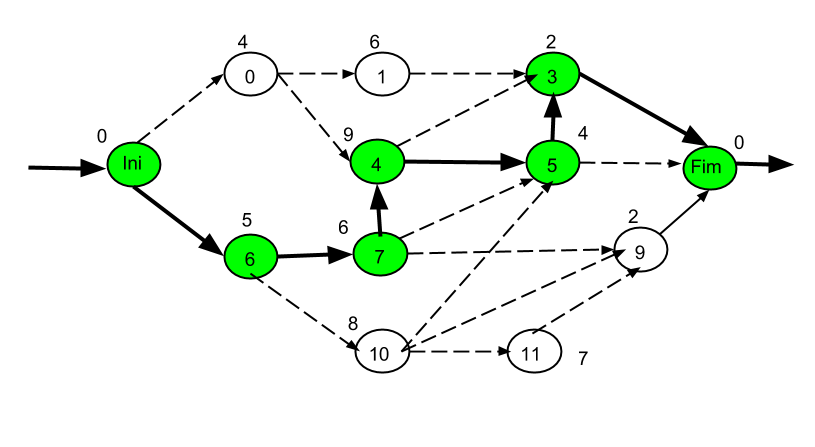
\includegraphics[scale=0.5]{./img/p1_caminho_critico}
\caption{Grafo com indicação do caminho crítico obtido. Os valores em cada nó representam a duração (em unidades de tempo) da respetiva atividade}
\label{p1:fig:caminho_critico}
\end{figure}

Este resultado indica que as atividades 6,7,4,5 e 3 devem ser vigiadas de perto e deve-se tentar garantir que são executadas nos tempos previstos, sem atrasos, caso contrário todo o projeto será atrasado..

\section{Validação do Modelo}

Para validar os resultados, tanto na função objetivo como nas restrições,
substituímos os valores das variáveis de decisão pelo valor que estas tomam na
solução que o lp\_solve indica como ótima. A ideia é verificar que os valores das
variáveis de decisão obtidos confirmam o valor da função objetivo obedecendo
a todas as restrições.

Para evitar ao máximo o erro humano, a substituição de variáveis foi feita
recorrendo a ferramentas que auxiliaram a substituição automática das variáveis
pelo seu valor.

\subsection{Variáveis de Decisão}

No resultado obtido todas as variáveis são de facto binárias, tomam apenas
o valor de 0 ou 1, tal como esperado.

\subsection{Função objetivo}

Depois da substituição das variáveis pelo seu valor, a função objetivo
fica:\\[0.5cm]

$0*0+0*1+4*0+4*0+6*0+2*1+9*0+9*1+4*1+4*0+5*1
+5*0+6*1+6*0+6*0+2*0+8*0+8*0+8*0+7*0 = 26$\\[0.5cm]

Inserindo a expressão numa calculadora verifica-se que a expressão é igual a 26,
o que confirma o resultado obtido com o \textit{lp\_solve}.

\subsection{Restrições}

\begin{itemize}

\item Nodo Inicio 

$1-X_{ini\_6} - X_{ini\_0} = 0$

$1 - 1 - 0 = 0$

\item Nodo 0 

$X_{ini\_0}-X_{0\_1}-X_{0\_4} = 0$

$0 - 0 - 0 = 0$

\item Nodo 1 

$	X_{0\_1}-X_{1\_3} = 0$

$0 - 0 = 0$

\item Nodo 3 

$	X_{1\_3} + X_{4\_3} + X_{5\_3}-X_{3\_fim} = 0$

$0 + 0 + 1 - 1 = 0$

\item Nodo 4 

$	X_{0\_4} + X_{7\_4} - X_{4\_3} - X_{4\_5} = 0$

$0 + 1 - 0 - 1= 0$

\item Nodo 5 

$X_{4\_5} + X_{7\_5} + X_{10\_5} - X_{5\_3} - X_{5\_fim} = 0$

$1 + 0 + 0 - 1 - 0 = 0$

\item Nodo 6 

$X_{ini\_6} - X_{6\_7} - X_{6\_10} = 0$

$1 - 1 - 0 = 0$

\item Nodo 7 

$X_{6\_7}- X_{7\_4}- X_{7\_5} - X_{7\_9} = 0$

$1 - 1 - 0 - 0 = 0$

\item Nodo 9 

$X_{7\_9} + X_{10\_9} + X_{11\_9} - X_{9\_fim} = 0$

$0 + 0 + 0 - 0 = 0$

\item Nodo 10 

$X_{6\_10} - X_{10\_5} - X_{10\_9} - X_{10\_11} = 0$

$0 - 0 - 0 - 0 = 0$

\item Nodo 11 

$X_{10\_11} - X_{11\_9} = 0$

$0 - 0 = 0$

\item Nodo Fim 

$X_{3\_fim} + X_{5\_fim} + X_{9\_fim} - 1 = 0$

$1 + 0 + 0 - 1 = 0$

\end{itemize}

Assim conclui-se que todas as restrições são respeitadas.







